\onecolumn

\begin{appendices}

\newtheorem{innercustomgeneric}{\customgenericname}
\providecommand{\customgenericname}{}
\newcommand{\newcustomtheorem}[2]{%
  \newenvironment{#1}[1]
  {%
   \renewcommand\customgenericname{#2}%
   \renewcommand\theinnercustomgeneric{##1}%
   \innercustomgeneric
  }
  {\endinnercustomgeneric}
}

\newcustomtheorem{customthm}{Theorem}
\newcustomtheorem{customlemma}{Lemma}


\renewcommand{\qedsymbol}{$\blacksquare$}
\newcommand{\R}[0]{\mathbb{R}}
\newcommand{\Prob}[1]{\mathbf{P}\left( #1 \right) }
\newcommand{\Exv}[1]{\mathbb{E}\left[ #1 \right]}
\newcommand{\Exvud}[2]{\mathbb{E}_{#1}\left[ #2 \right]}
% \newcommand*{\Exv}{\mathbb{E}}
\newcommand{\norm}[1]{\left\| #1 \right\|}
\newcommand{\Abs}[1]{\left| #1 \right| }

% \nipsfinalcopy is no longer used
% \maketitle
\section{Overview}
The appendix will contain full proofs for all theorems and lemmas in the main paper, implementation details for all the experiments, statistics for the figures, and some additional results combining SWALP with other methods.
The proof for Theorem~\ref{thm:quadratic} will be presented in Sec~\ref{sec:appendix-thm-quadratic}. 
The proof for Lemma~\ref{lemmaNoiseBall} will be presented in Sec~\ref{sec:appendix-lemma}.
The proof for Theorem~\ref{thm:SWALP} will be shown in Sec~\ref{sec:thm4.3}.
The proof for Theorem~\ref{thm:lower-bound} will be shown in Sec~\ref{sec:thm-lowerbound}.
The implementation details of the linear regression and the logistic regression experiments will be in Sec~\ref{sec:linreg} and Sec~\ref{sec:logreg} respectively.
The implementation details for deep learning experiments will be presented in Sec~\ref{sec:dlexp}.
We show results combining SWALP with WAGE~\cite{WAGE} in Sec~\ref{sec:wage-swalp}.
In the rest sections, we will provide numbers used for the figure.


\section{Proof for Theorem~\ref{thm:quadratic}}\label{sec:appendix-thm-quadratic}

Here, we provide a more detailed proof of Theorem~\ref{thm:quadratic}.

Consider a quadratic objective function $f(w) = (w - w^*)^T A (w - w^*) / 2$ for some $A \in \mathbb{R}^{d \times d}$ and $w^* \in \mathbb{R}^d$ is the optimal solution.
Assume $A \succeq \mu I$, where $\mu > 0$ is the strong convexity parameter of this function.
Suppose that we want to minimize $f$ using SWALP with gradient samples $\nabla \tilde f(w)$ that satisfy $\mathbb{E}[\nabla \tilde f(w)] = \nabla f(w) = A (w - w^*)$.
Suppose that the variance of these samples always satisfies $\mathbb{E}[\| \nabla \tilde f(w) - \nabla f(w) \|_2^2] \le \sigma^2$ for some constant $\sigma$; this is a standard assumption used in the analysis of SGD.
Then we can prove the following:

\begin{customthm}{\ref{thm:quadratic}}
Suppose we run SWALP under the above assumptions with a cycle length $c$ and $0 < \alpha < \frac{1}{2}\|A\|_2$.
The expected squared distance to the optimum of SWALP's output is bounded by
\[{
\mathbb{E}\left[\|\bar{w}_T - w^*\|^2 \right]
\leq
\frac{\|w_0 - w^*\|^2}{\alpha^2\mu^2T^2} + 
\frac{c(\alpha^2\sigma^2 + \frac{\delta^2d}{4})}{\alpha^2\mu^2T}
}\]
\end{customthm}

\begin{proof}
We start by rewriting the iterates of low-precision SGD as
\begin{align*}
    w_{t+1} &= Q_\delta(w_t - \alpha \nabla \tilde{f}(w_t)) \\
    &= w_t - \alpha A(w_t-w^*) + \zeta_t
\end{align*}
where $\zeta_t$, the error term is explicitly defined as
\begin{align*}
    \zeta_t &= Q_\delta(w_t - \alpha \nabla \tilde{f}(w_t)) - w_t + \alpha A(w_t - w^*) \\
    &= Q_\delta(w_t - \alpha \nabla \tilde{f}(w_t)) - w_t + \alpha A(w_t - w^*) + \alpha \nabla \tilde{f}(w_t) - \alpha \nabla \tilde{f}(w_t) \\
    &= \alpha(A(w_t - w^*) - \nabla\tilde{f}(w_t)) + Q_\delta(w_t - \alpha \nabla \tilde{f}(w_t)) - (w_t - \alpha \nabla \tilde{f}(w_t)).
\end{align*}

We know that $\mathbb{E}[\zeta_i] = 0$ since
\begin{align*}
    \mathbb{E}[\zeta_t] &= \mathbb{E}[\alpha(A(w_t - w^*) - \nabla\tilde{f}(w_t)) + Q_\delta(w_t - \alpha \nabla \tilde{f}(w_t)) - (w_t - \alpha \nabla \tilde{f}(w_t))] \\
    &=\alpha \big(A(w_t - w^*) - \mathbb{E}[\nabla\tilde{f}(w_t)]\big) + \big(\mathbb{E}[Q_\delta(w_t - \alpha \nabla \tilde{f}(w_t))] - (w_t - \alpha \nabla \tilde{f}(w_t))\big) \\
    &= 0.
\end{align*}
Moreover, due to independence, we can bound the variance of $\zeta_t$ as
\begin{align*}
    \mathbb{E}\left[ \| \zeta_t \|^2 \right] 
    &= 
    \mathbb{E}\left[ \| \alpha(A(w_t - w^*) - \nabla\tilde{f}(w_t)) \|^2 \right] 
    + 
    \mathbb{E}\left[ \| Q_\delta(w_t - \alpha \nabla \tilde{f}(w_t)) - (w_t - \alpha \nabla \tilde{f}(w_t)) \|^2 \right] \\
    &\leq
    \alpha^2\sigma^2 + \frac{\delta^2 d}{4}
\end{align*}
where $d$ is the dimension of the solution and $\sigma$ is an upper bound for $A(w_t - w^*)$.
Then 
\begin{align*}
    w_{t+1} - w^* &= w_t - w^* - \alpha A(w-w^*) + \zeta_t \\
    &= (I-\alpha A)(w_t - w^*) + \zeta_t
\end{align*}
Expanding this formula we will have
\begin{align*}
    w_t - w^* = (I-\alpha A)^t(w_0-w^*) + \displaystyle\sum_{i=0}^{t-1} (I-\alpha A)^{t-i-1}\zeta_i
\end{align*}
Computing the distance from the average $\bar{w}_T$ to $w^*$, we get
\begin{align*}
    \bar{w}_K - w^* &= \frac{1}{K}\displaystyle\sum_{t=1}^K w_{ct} - w^* \\
    &=\frac{1}{K}\displaystyle\sum_{t=1}^K\bigg(
    (I-\alpha A)^{ct}(w_0-w^*) + \displaystyle\sum_{i=0}^{ct-1} (I-\alpha A)^{ct-i-1}\zeta_i
    \bigg) \\
    &=\frac{1}{K}\bigg(\displaystyle\sum_{t=1}^K(I-\alpha A)^{ct}\bigg)(w_0-w^*) 
    + \frac{1}{K}\displaystyle\sum_{t=1}^K\displaystyle\sum_{i=0}^{ct-1} (I-\alpha A)^{ct-i-1}\zeta_i. \\
\end{align*}
Note that the first term is a constant; let that be $\chi_K$. Now analyzing the variance:
\begin{align*}
\mathbb{E}\left[\|\bar{w}_K - w^*\|^2\right] &= \mathbb{E}\left[
    \left\|\chi_K + \frac{1}{K}\displaystyle\sum_{t=1}^K\displaystyle\sum_{i=0}^{ct-1} (I-\alpha A)^{ct-i-1}\zeta_i \right\|^2
\right] \\
&= \|\chi_K\|^2 + \mathbb{E}\left[
    \left\|\frac{1}{K}\displaystyle\sum_{t=1}^K\displaystyle\sum_{i=0}^{ct-1} (I-\alpha A)^{ct-i-1}\zeta_i \right\|^2
\right]
\\&\hspace{4em}+ 
    \frac{2}{K}\chi_K^T\displaystyle\sum_{t=1}^K\displaystyle\sum_{i=0}^{ct-1} (I-\alpha A)^{ct-i-1}\mathbb{E}[\zeta_i] \\
&= \|\chi_K\|^2 + \mathbb{E}\left[
    \left\|\frac{1}{K}\displaystyle\sum_{t=1}^K\displaystyle\sum_{i=0}^{ct-1} (I-\alpha A)^{ct-i-1}\zeta_i \right\|^2
\right] \\ 
&= \|\chi_K\|^2 + \frac{1}{K^2} \mathbb{E}\left[
    \left\|\sum_{i=0}^{cK-1}\displaystyle\sum_{t=\lfloor i/c \rfloor + 1}^{K} (I-\alpha A)^{ct-i-1}\zeta_i \right\|^2
\right] 
\end{align*}
Now leveraging the fact that the $\zeta_i$ are zero-mean and independent, we get
\begin{align*}
\mathbb{E}\left[\|\bar{w}_K - w^*\|^2\right]
&= \|\chi_K\|^2 + \frac{1}{K^2} \sum_{i=0}^{cK-1} \mathbb{E}\left[
    \left\| \sum_{t=\lfloor i/c \rfloor + 1}^{K} (I-\alpha A)^{ct-i-1}\zeta_i \right\|^2
\right] \\
&\leq \|\chi_K\|^2 + \frac{1}{K^2} \sum_{i=0}^{cK-1} \left\| \sum_{t=\lfloor i/c \rfloor + 1}^{K} (I-\alpha A)^{ct-i-1} \right\|_2^2 \mathbb{E}\left[
    \left\| \zeta_i \right\|^2
\right]  \\
&\leq \|\chi_K\|^2 + \frac{1}{K^2} \sum_{i=0}^{cK-1} \left\| \sum_{j=0}^{\infty} (I-\alpha A)^j \right\|_2^2 \mathbb{E}\left[
    \left\| \zeta_i \right\|^2
\right] 
\end{align*}
where in the final step the inequality holds because every term in the finite sum within the norm also must appear in the infinite sum.
Next, since $0 < \alpha < \|A\|_2/2$, we know the series sum $ \sum_{j=0}^{\infty} (I-\alpha A)^{j}$ will converge, and we have:
\begin{align*}
\left\| \sum_{j=0}^{\infty} (I-\alpha A)^{j} \right\|_2^2
= 
\left\|(I - (I-\alpha A))^{-1}\right\|_2^2 
=
\left\|\frac{1}{\alpha}A^{-1} \right\|_2^2
\leq
\frac{1}{\alpha^2\mu^2}.
\end{align*}

Putting this back we get,
\begin{align*}
\mathbb{E}[||\bar{w}_K - w^*||^2]
&\leq \|\chi_K\|^2 + 
    \frac{1}{K^2\alpha^2\mu^2} \displaystyle\sum_{i=0}^{cK-1}\mathbb{E}[\|\zeta_i\|^2]  \\
&\leq \|\chi_K\|^2 + 
    \frac{c}{K\alpha^2\mu^2} \left(\alpha^2\sigma^2 + \frac{\delta^2d}{4} \right).
\end{align*}

Finally, we analyze the term $\|\chi_K\|^2$, we will get
\begin{align*}
\|\chi_K\|^2 &= \left\|\frac{1}{K}\big(\displaystyle\sum_{t=1}^K(I-\alpha A)^{ct}\big)(w_0-w^*)\right\|^2 \\
&\leq \frac{1}{K^2}\left\|\displaystyle\sum_{t=1}^K(I-\alpha A)^{ct}\right\|_2^2 \  \left\|w_0 -w^*\right\|^2 \\
&\leq \frac{1}{K^2}\left\|\displaystyle\sum_{t=1}^\infty (I-\alpha A)^t\right\|_2^2 \ \left\|w_0 -w^*\right\|^2 \\
&= \frac{1}{K^2}\left\|(I - (I - \alpha A))^{-1}\right\|_2^2 \ \left\|w_0 -w^*\right\|^2 \\
&= \frac{1}{K^2}\left\|\frac{1}{\alpha}A^{-1}\right\|_2^2 \ \left\|w_0 -w^*\right\|^2 \\
&\leq \frac{1}{K^2\alpha^2\mu^2} \ \left\|w_0 -w^*\right\|^2
\end{align*}

Putting this bound together, we get:
\begin{align*}
    \mathbb{E}[||\bar{w}_K - w^*||^2]
&\leq \frac{1}{K^2\alpha^2\mu^2} \ \|w_0 -w^*\|^2 + 
    \frac{c}{K\alpha^2\mu^2} \left(\alpha^2\sigma^2 + \frac{\delta^2d}{4} \right)
\end{align*}
which is what we wanted to show.
\end{proof}



\section{Proof for Lemma~\ref{lemmaNoiseBall}}\label{sec:appendix-lemma}

Let's start by analyzing an update step
\[
  w_{t+1} = Q_{\delta}\left( w_t - \alpha \nabla \tilde f_t(w_t) \right)
\]
where $\Exv{\tilde f_t} = f$ and $f$ is strongly convex with parameter $\mu$, Lipschitz continuous with parameter $L$, and has a global minimum at $w^*$.
Further suppose that
\[
  \norm{ \nabla \tilde f_t(w) - \nabla f(w) } \le G
\]
for all $w \in \mathbb{R}^d$.

\begin{customlemma}{\ref{lemmaNoiseBall}}
  Under the above conditions, suppose that we run with step size
  \[
    \alpha
    =
    \sqrt{ \frac{\delta^2 d}{G^2} }
  \]
  and further suppose that $\delta$ is small enough that this step size satisfies
  $(1 - 2 \alpha \mu + \alpha^2 L)^2 \le 1 - 2 \alpha \mu$ and $\alpha \mu < 1$.
  Suppose that we run low-precision SGD for a number of time steps that is at least
  \[
    T
    \ge
    \frac{2 G}{\mu \delta \sqrt{d}} \log\left( \frac{\mu \norm{w_0 - w^*}^2}{44 G \delta \sqrt{d}} \right).
  \]
  Then
  \[
    \Exv{ \norm{w_T - w^*}^4 }
    \le
    \frac{44^2 G^2 \delta^2 d}{\mu^2}.
  \]
  \label{lemmaNewSingleIterBound}
\end{customlemma}

\begin{proof}
We start by bounding the quantity we are interested in at the next time step with
\begin{align*}
  \norm{w_{t+1} - w^*}^4
  &=
  \norm{Q_{\delta}\left( w_t - \alpha \nabla \tilde f_t(w_t) \right) - w^*}^4 \\
  &=
  \norm{w_t - w^* - \alpha \nabla f(w_t) - \left(
    w_t - \alpha \nabla \tilde f_t(w_t)
    -
    Q_{\delta}\left( w_t - \alpha \nabla \tilde f_t(w_t) \right)
    +
    \alpha \nabla \tilde f_t(w_t)
    -
    \alpha \nabla f(w_t)
  \right) }^4.
\end{align*}
If we define
\[
  u_t
  =
  -\left(
  w_t - \alpha \nabla \tilde f_t(w_t)
  -
  Q_{\delta}\left( w_t - \alpha \nabla \tilde f_t(w_t) \right)
  +
  \alpha \nabla \tilde f_t(w_t)
  -
  \alpha \nabla f(w_t)\right),
\]
then since we use unbiased rounding, $\Exv{u_t} = 0$.
And so,
\begin{align*}
  \Exv{ \norm{w_{t+1} - w^*}^4 }
  &=
  \Exv{ \norm{w_t - w^* - \alpha \nabla f(w_t) + u_t }^4 } \\
  &=
  \Exv{ \norm{w_t - w^* - \alpha \nabla f(w_t) }^4 }
  +
  \Exv{ 4 \norm{w_t - w^* - \alpha \nabla f(w_t) }^2
  u_t^T \left(w_t - w^* - \alpha \nabla f(w_t)\right) }
  \\&\hspace{2em}+
  \Exv{ 2 \norm{w_t - w^* - \alpha \nabla f(w_t) }^2 \norm{u_t}^2 }
  +
  \Exv{ 4 \left( u_t^T \left(w_t - w^* - \alpha \nabla f(w_t)\right) \right)^2 }
  \\&\hspace{2em}+
  \Exv{ 4 \norm{u_t}^2 u_t^T \left(w_t - w^* - \alpha \nabla f(w_t)\right) }
  +
  \Exv{ \norm{u_t}^4 } \\
  &=
  \Exv{ \norm{w_t - w^* - \alpha \nabla f(w_t) }^4 }
  +
  \Exv{ 2 \norm{w_t - w^* - \alpha \nabla f(w_t) }^2 \norm{u_t}^2 }
  \\&\hspace{2em}+
  \Exv{ 4 \left( u_t^T \left(w_t - w^* - \alpha \nabla f(w_t)\right) \right)^2 }
  +
  \Exv{ 4 \norm{u_t}^2 u_t^T \left(w_t - w^* - \alpha \nabla f(w_t)\right) }
  +
  \Exv{ \norm{u_t}^4 } \\
  &\le
  \Exv{ \norm{w_t - w^* - \alpha \nabla f(w_t) }^4 }
  +
  \Exv{ 6 \norm{w_t - w^* - \alpha \nabla f(w_t) }^2 \norm{u_t}^2 }
  \\&\hspace{2em}+
  \Exv{ 4 \norm{w_t - w^* - \alpha \nabla f(w_t) } \norm{u_t}^3 }
  +
  \Exv{ \norm{u_t}^4 }.
\end{align*}
From Holder's inequality, we know that
\[
  \Exv{X^m Y^n}
  \le
  \Exv{\Abs{X}^{m+n}}^{\frac{m}{m+n}} \Exv{\Abs{Y}^{m+n}}^{\frac{n}{m+n}},
\]
so
\begin{align*}
  \Exv{ \norm{w_{t+1} - w^*}^4 }
  &\le
  \Exv{ \norm{w_t - w^* - \alpha \nabla f(w_t) }^4 }
  +
  6 \Exv{ \norm{w_t - w^* - \alpha \nabla f(w_t) }^4 }^{\frac{1}{2}}
  \Exv{ \norm{u_t}^4 }^{\frac{1}{2}}
  \\&\hspace{2em}+
  4 \Exv{ \norm{w_t - w^* - \alpha \nabla f(w_t) }^4 }^{\frac{1}{4}}
  \Exv{ \norm{u_t}^4 }^{\frac{3}{4}}
  +
  \Exv{ \norm{u_t}^4 }.
\end{align*}
Now, it's a well known result for convex functions that
\begin{align*}
  \norm{w_t - w^* - \alpha \nabla f(w_t) }^2
  &=
  \norm{w_t - w^*}^2 
  - 
  2\alpha (w_t - w^*)^T \left( \nabla f(w_t) - \nabla f(w^*) \right)
  +
  \norm{ \nabla f(w_t) - \nabla f(w^*) }^2 \\
  &\le
  \norm{w_t - w^*}^2 
  - 
  2 \alpha \mu \norm{w_t - w^*}^2 
  +
  \alpha^2 L \norm{w_t - w^*}^2 \\
  &=
  (1 - 2 \alpha \mu + \alpha^2 L) \norm{w_t - w^*}^2,
\end{align*}
so
\[
  \norm{w_t - w^* - \alpha \nabla f(w_t) }^4
  \le
  (1 - 2 \alpha \mu + \alpha^2 L)^2 \norm{w_t - w^*}^4.
\]
On the other hand, we can bound the magnitude of $u$ with
\begin{align*}
  \norm{ u_t }
  &=
  \norm{ 
    w_t - \alpha \nabla \tilde f_t(w_t)
    -
    Q_{\delta}\left( w_t - \alpha \nabla \tilde f_t(w_t) \right)
    +
    \alpha \nabla \tilde f_t(w_t)
    -
    \alpha \nabla f(w_t)
    } \\
  &\le
  \norm{ 
    w_t - \alpha \nabla \tilde f_t(w_t)
    -
    Q_{\delta}\left( w_t - \alpha \nabla \tilde f_t(w_t) \right)
  }
  +
  \norm{
    \alpha \nabla \tilde f_t(w_t)
    -
    \alpha \nabla f(w_t)
  } \\
  &\le
  \delta \sqrt{d}
  +
  \alpha G.
\end{align*}
If we define $C = \delta \sqrt{d} + \alpha G$, then $\norm{ u_t } \le C$, and so
\begin{align*}
  \Exv{ \norm{w_{t+1} - w^*}^4 }
  &\le
  (1 - 2 \alpha \mu + \alpha^2 L)^2 \Exv{\norm{w_t - w^*}^4}
  +
  6 (1 - 2 \alpha \mu + \alpha^2 L) \Exv{\norm{w_t - w^*}^4}^{\frac{1}{2}}
  C^2
  \\&\hspace{2em}+
  4 \sqrt{1 - 2 \alpha \mu + \alpha^2 L} \cdot \Exv{\norm{w_t - w^*}^4}^{\frac{1}{4}}
  C^3
  +
  C^4 \\
  &\le
  (1 - 2 \alpha \mu + \alpha^2 L)^2 \Exv{\norm{w_t - w^*}^4}
  +
  6 C^2 \Exv{\norm{w_t - w^*}^4}^{\frac{1}{2}}
  +
  4 C^3 \Exv{\norm{w_t - w^*}^4}^{\frac{1}{4}}
  +
  C^4.
\end{align*}
Next, suppose we choose $\alpha$ small enough that $(1 - 2 \alpha \mu + \alpha^2 L)^2 \le 1 - 2 \alpha \mu$. Then,
\begin{align*}
  \Exv{ \norm{w_{t+1} - w^*}^4 }
  &\le
  (1 - 2 \alpha \mu) \Exv{\norm{w_t - w^*}^4}
  +
  6 C^2 \Exv{\norm{w_t - w^*}^4}^{\frac{1}{2}}
  +
  4 C^3 \Exv{\norm{w_t - w^*}^4}^{\frac{1}{4}}
  +
  C^4.
\end{align*}
Now, suppose that $\Exv{\norm{w_t - w^*}^4}$ is large enough that
\[
  \Exv{\norm{w_t - w^*}^4} \ge C^4.
\]
Then,
\begin{align*}
  \Exv{ \norm{w_{t+1} - w^*}^4 }
  &\le
  (1 - 2 \alpha \mu) \Exv{\norm{w_t - w^*}^4}
  +
  11 C^2 \Exv{\norm{w_t - w^*}^4}^{\frac{1}{2}}.
\end{align*}
And if we further suppose that $\Exv{\norm{w_t - w^*}^4}$ is large enough that
\[
  \alpha \mu \Exv{\norm{w_t - w^*}^4} \ge 11 C^2 \Exv{\norm{w_t - w^*}^4}^{\frac{1}{2}},
\]
which is equivalent to
\[
  \Exv{\norm{w_t - w^*}^4} \ge \left( \frac{11 C^2}{\alpha \mu} \right)^2,
\]
then
\begin{align*}
  \Exv{ \norm{w_{t+1} - w^*}^4 }
  &\le
  (1 - \alpha \mu) \Exv{\norm{w_t - w^*}^4}.
\end{align*}
So we've shown that $\Exv{ \norm{w_{t+1} - w^*}^4 }$ decreases exponentially until it no longer satisfies one of our two suppositions, which,  
as long as $\alpha \mu < 11$, will be
\[
  \Exv{\norm{w_t - w^*}^4} \ge \left( \frac{11 C^2}{\alpha \mu} \right)^2.
\]
In other words, independently of any suppositions on the magnitude of $\Exv{ \norm{w_{t+1} - w^*}^4 }$ (but still assuming $\alpha \mu < 11$), it will hold that
\begin{align*}
  \Exv{ \norm{w_{t+1} - w^*}^4 }
  &\le
  (1 - \alpha \mu) \max\left( \Exv{\norm{w_t - w^*}^4}, \left( \frac{11 C^2}{\alpha \mu} \right)^2 \right).
\end{align*}
And applying this recursively,
\begin{align*}
  \Exv{ \norm{w_T - w^*}^4 }
  &\le
  \max\left( (1 - \alpha \mu)^T \norm{w_0 - w^*}^4, \left( \frac{11 C^2}{\alpha \mu} \right)^2 \right) \\
  &\le
  \max\left( \exp(- \alpha \mu T) \norm{w_0 - w^*}^4, \left( \frac{11 C^2}{\alpha \mu} \right)^2 \right).
\end{align*}
It follows that, as long as $T$ is large enough that
\[
  \exp(- \alpha \mu T) \norm{w_0 - w^*}^4 \le \left( \frac{11 C^2}{\alpha \mu} \right)^2,
\]
which will occur when
\[
  T \ge \frac{2}{\alpha \mu} \log\left( \frac{\alpha \mu \norm{w_0 - w^*}^2}{11 C^2} \right),
\]
we will get 
\begin{align*}
  \Exv{ \norm{w_T - w^*}^4 }
  &\le
  \left( \frac{11 C^2}{\alpha \mu} \right)^2.
\end{align*}
Next, we simplify this fraction.
\begin{align*}
  \frac{C^2}{\alpha \mu}
  &=
  \frac{\left( \delta \sqrt{d} + \alpha G \right)^2}{\alpha \mu}.
\end{align*}
If we set $\alpha = G^{-1} \delta \sqrt{d}$ then
\begin{align*}
  \frac{C^2}{\alpha \mu}
  &=
  \frac{\left( \delta \sqrt{d} + G^{-1} \delta \sqrt{d} \cdot G \right)^2}{G^{-1} \delta \sqrt{d} \mu} \\
  &=
  \frac{\left( 2 \delta \sqrt{d} \right)^2 \cdot G}{\delta \sqrt{d} \mu} \\
  &=
  \frac{4 G \delta \sqrt{d}}{\mu}.
\end{align*}
It follows that our bound on $T$ becomes
\[
  T \ge \frac{2 G}{\mu \delta \sqrt{d}} \log\left( \frac{\mu \norm{w_0 - w^*}^2}{44 G \delta \sqrt{d}} \right),
\]
and our bound on $\Exv{ \norm{w_T - w^*}^4 }$ becomes
\begin{align*}
  \Exv{ \norm{w_T - w^*}^4 }
  &\le
  \left( \frac{44 G \delta \sqrt{d}}{\mu} \right)^2 \\
  &=
  \frac{44^2 G^2 \delta^2 d}{\mu^2}.
\end{align*}
This is what we wanted to prove.
\end{proof}

\newpage


\section{Proof for Theorem~\ref{thm:SWALP}}\label{sec:thm4.3}

\begin{customthm}{\ref{thm:SWALP}}
Suppose that we run SWALP under the above conditions, with the parameters specified in Lemma~\ref{lemmaNewSingleIterBound}.
Also, suppose that we first run a warm-up phase and start averaging at some point $w_0$ after enough iterations of low-precision SGD such that the bound of Lemma~\ref{lemmaNewSingleIterBound} is already guaranteed to apply for this and all subsequent iterates.
Let $\bar{w}$ be the output of SWALP using cycle length $c$, and $\gamma = min(\alpha^2\mu^2c^2,1)$.
The expected squared distance to the optimum of the output of SWALP is bounded by
\begin{align*}
% {\textstyle
    \mathbb{E}[\|\bar{w} - w^*\|^2] \leq
    \frac{5808 M^2G^2\delta^2 d}{\mu^4} + 
    \frac{6 G^2 c}{\mu^2 T} +
    \frac{528 \sqrt{d}\delta G^3 c^2}{\gamma\mu T^2}.
% }
\end{align*}
\end{customthm}


\begin{proof}
Consider the case that $\bar{w}$ is output after $K$ averagings. Therefore, we could assume $cK \leq T < cK+c$, and $\bar{w}=\frac{1}{K}\sum_{t=0}^{K-1} w_{tc}$.
From rearranging the SGD update step, we have
\begin{align*}
  w_t - w_{t+1}
  &=
  Q_{\delta}\left(\alpha \nabla \tilde f_t(w_t) \right) \\
  &=
  \alpha H (w_t - w^*)
  +
  \alpha \left(
    \nabla f(w_t)
    -
    H (w_t - w^*)
  \right)
  +
  Q_{\delta}\left(\alpha \nabla \tilde f_t(w_t) \right)
  -
  \alpha \nabla f(w_t)
\end{align*}
where we let $H$ denote $H = \nabla^2 f(w^*)$.
For simplicity of the presentation, we let
\begin{align*}
    \phi_t &= \nabla f(w_t) - H ( w_t - w^*) \\
    \psi_t &= Q_\delta(\alpha \nabla \tilde{f}_t(w_t)) - \alpha \nabla f(w_t) \\
    \eta_t &= -\alpha \left(\nabla f(w_t) - H (w_t - w^*) \right)
              - Q_{\delta}\left(\alpha \nabla \tilde f_t(w_t) \right)
              + \alpha \nabla f(w_t) \\
           &= \alpha \phi_t + \psi_t
\end{align*}
Then  we can re-arrange the terms as following:
\begin{align*}
    w_{t+1} &= w_t - \alpha H(w_t - w^*) - \eta_t \\
    w_{t+1} - w^* &= (w_t - w^*) - \alpha H ( w_t - w^* ) - \eta_t \\
                  &= (I - \alpha H) (w_t - w^*) - \eta_t \\
    w_{t+c} - w^* &= (I - \alpha H)^c ( w_t - w^*) - \sum_{i=0}^{c-1} \eta_{t+i}(I-\alpha H)^{c-u-1} \\
    w_t - w_{t+c} &= (I - (I - \alpha H)^c) ( w_t - w^*) + \sum_{i=0}^{c-1}(I - \alpha H)^{c-i-1}\eta_{t+i} \\
    w_0 - w_{cK} &= \sum_{t=0}^{K-1}(I - (I-\alpha H)^c)(w_{tc} - w^*) + \sum_{t=0}^{K-1} \sum_{i=0}^{c-1} (I - \alpha H)^{c-i-1} \eta_{ct+i} \\
    \frac{1}{K}(w_0 - w_{cK}) &= 
        \frac{1}{K}\sum_{t=0}^{K-1}(I - (I-\alpha H)^c)(w_{tc} - w^*) + 
        \frac{1}{K}\sum_{t=0}^{K-1} \sum_{i=0}^{c-1} (I - \alpha H)^{c-i-1} \eta_{ct+i} \\
        &= 
        (I - (I-\alpha H)^c) \frac{1}{K}\sum_{t=0}^{K-1}(w_{tc} - w^*) + 
        \frac{1}{K}\sum_{t=0}^{K-1} \sum_{i=0}^{c-1} (I - \alpha H)^{c-i-1} \eta_{ct+i} \\
\end{align*}
We know $\bar{w} = \frac{1}{K}\sum_{t=0}^{K-1} w_{tc}$ and $cK \leq T < cK+c$. So $\frac{1}{K}\sum_{t=0}^{K-1}(w_{tc} - w^*) = \bar{w} - w^*$. 
\begin{align*}
\bar{w} - w^* &= (I - (I - \alpha H)^c)^{-1} \left[ 
    \frac{1}{K}(w_0 - w_{cK}) + \frac{1}{K}\sum_{t=0}^{K-1}\sum_{i=0}^{c-1} (I-\alpha H)^{c-i-1} \eta_{ct+i}
\right]
\end{align*}

Bounding the expected norm of $\bar{w} - w^*$, we get
\begin{align*}
    \Exv{\|\bar{w} - w^*\|} & \leq \frac{1}{K}\Exv{\left\|(I-(I - \alpha H)^c)^{-1} (w_0 - w_{cK})\right\|} \\
                            & \quad + \frac{\alpha}{K} \Exv{\left\|\sum_{i=0}^{c-1} (I - (I-\alpha H)^c)^{-1} (I - \alpha H)^{c-i-1} \phi_{ct+i}\right\|} \\ 
                            & \quad + \Exv{\left\|\frac{1}{K}\sum_{t=0}^{K-1}\sum_{i=0}^{c-1}(I - (I - \alpha H)^c)^{-1} (I - \alpha H )^{c-i-1} \psi_{ct+i}\right\|}
\end{align*}
Applying the inequality $(x+y+z)^2 \leq 3x^2+3y^2+3z^2$, we get
\begin{align*}
    \Exv{\|\bar{w} - w^*\|^2} & \leq \frac{3}{K^2}\Exv{\left\|(I-(I - \alpha H)^c)^{-1} (w_0 - w_{cK})\right\|^2} \\
                            & \quad + 3 \alpha^2\left(\frac{1}{K} \Exv{\left\|\sum_{i=0}^{c-1} (I - (I-\alpha H)^c)^{-1} (I - \alpha H)^{c-i-1} \phi_{ct+i}\right\|}\right)^2 \\ 
                            & \quad + 3\Exv{\left\|\frac{1}{K}\sum_{t=0}^{K-1}\sum_{i=0}^{c-1}(I - (I - \alpha H)^c)^{-1} (I - \alpha H )^{c-i-1} \psi_{ct+i}\right\|^2}
\end{align*}
We will now bound each of these three terms separately, starting with the first term:
\begin{align*}
    \frac{3}{K^2}\Exv{\left\| (I - (I - \alpha H)^c)^{-1} ( w_0 - w_{cK}) \right\|^2} 
    & \leq \frac{3}{K^2}\left\| (I - (I - \alpha H)^c)^{-1}\right\|_2^2 \Exv{\|w_0 - w_{cK}\|^2}
\end{align*}
By the result of Lemma~\ref{lemmaNoiseBall}, and Jensen's inequality, we will have
\begin{align*}
    \Exv{\|w_t - w^*\|^2} \leq \Exv{\|w_t - w^*\|^4}^{\frac{1}{2}} \leq \frac{44G\delta \sqrt{d}}{\mu}
\end{align*}
for any fixed $t$ during the executation of the algorithm (after the warm-up period). It follows that
\begin{align*}
    \Exv{\|w_0 - w_K\|^2}] 
    &\leq 2\Exv{\|w_K - w^*\|^2} + 2 \Exv{\|w_0 - w^*\|^2} \\
    &\leq \frac{176 G \delta \sqrt{d}}{\mu \alpha^2 K^2} = \frac{176 G^3}{\mu \delta \sqrt{d} K^2}
\end{align*}
where the last line followed by substituting $\alpha = \sqrt{\frac{\delta^2 d}{G^2}}$ from Lemma~\ref{lemmaNoiseBall}.
Since $H \succeq \mu I$, so $\|H\|_2 \geq \mu$. We have
\begin{align*}
    \|(I - (I - \alpha H)^c)^{-1}\|_2^2 \leq  (1 - (1 - \alpha \mu)^c)^{-2}
\end{align*}
Therefore, we get the following bound on the first term:
\begin{align*}
    \frac{3}{K^2}\Exv{\left\| (I - (I - \alpha H)^c)^{-1} ( w_0 - w_{cK}) \right\|^2} 
    & \leq \frac{1}{K^2}(1-(1-\alpha \mu)^c)^{-2}\frac{176 G\delta \sqrt{d}}{\mu}
\end{align*}
Note that if c is really small (i.e. $\alpha \mu c << 1$), then
\begin{align*}

    (1- (1- \alpha \mu)^c)^{-2} \leq \frac{1}{\alpha^2 \mu^2 c^2}
\end{align*}
If $c$ is large, then $(1-(1 - \alpha \mu)^c)^{-2} \rightarrow 1$, so we can bound it by 
\begin{align*}
    (1- (1- \alpha \mu)^c)^{-2} \leq \frac{1}{min(\alpha^2\mu^2c^2, 1)} = \frac{1}{\gamma}
\end{align*}
Therefore, the first term is then bounded by:
\begin{align*}
    \frac{3}{K^2}\Exv{\left\| (I - (I - \alpha H)^c)^{-1} ( w_0 - w_{cK}) \right\|^2} 
    & \leq \frac{528 G \delta \sqrt{d}}{\gamma \mu K^2}
\end{align*}

Now we proceed to bound the second term:
\begin{align*}
    & 3 \alpha^2\left(\frac{1}{K} \Exv{\left\|\sum_{i=0}^{c-1} (I - (I-\alpha H)^c)^{-1} (I - \alpha H)^{c-i-1} \phi_{ct+i}\right\|}\right)^2 \\
    &\quad \leq \frac{3\alpha^2}{K} \left( \sum_{t=0}^{K-1} \Exv{\left\|\sum_{i=0}^{c-1} (I - \alpha H)^{c-i-1} \phi_{ct+i}\right\|^2} \right) \left\| (I - (I - \alpha H)^c)^{-1} \right\|_2^2
\end{align*}
Analyzing the the expectation term, 
\begin{align*}
    & \Exv{\left\| \sum_{i=0}^{c-1} (I - \alpha H)^{c-i-1}\phi_{ct+i} \right\|^2} \\
    & \quad = \left( \sum_{i=0}^{c-1} (1 - \alpha \mu )^{c-i-1} \right)^2 \Exv{\left\| \frac{1}{\sum_{i=0}^{c-1}(1-\alpha \mu)^{c-i-1}}\sum_{i=0}^{c-1} \frac{(1-\alpha\mu)^{c-i-1}}{(1-\alpha\mu)^{c-i-1}}(I - \alpha H)^{c-i-1}\phi_{ct+i} \right\|^2} \\
    & \quad = \left( \sum_{i=0}^{c-1} (1 - \alpha \mu )^{c-i-1} \right)^2 
    \Exv{\left\| 
        \sum_{i=0}^{c-1} 
            \frac{(1-\alpha\mu)^{c-i-1}}{\sum_{i=0}^{c-1}(1-\alpha \mu)^{c-i-1}}
            \frac{(I - \alpha H)^{c-i-1}}{(1-\alpha\mu)^{c-i-1}}\phi_{ct+i} \right\|^2} \\
     & \quad \leq \left( \sum_{i=0}^{c-1} (1 - \alpha \mu )^{c-i-1} \right)^2 
        \sum_{i=0}^{c-1} \frac{(1-\alpha\mu)^{c-i-1}}{\sum_{i=0}^{c-1}(1-\alpha \mu)^{c-i-1}}
        \Exv{\left\| 
            \frac{(I - \alpha H)^{c-i-1}}{(1-\alpha\mu)^{c-i-1}}\phi_{ct+i} \right\|^2}
        \quad (\text{Jensen's inequality}) \\
    & \quad = \left( \sum_{i=0}^{c-1} (1 - \alpha \mu )^{c-i-1} \right)\sum_{i=0}^{c-1} (1 - \alpha \mu)^{c-i-1} \Exv{\left\|\frac{(I-\alpha H)^{c-i-1}}{(1-\alpha\mu)^{c-i-1}}\phi_{ct+i}\right\|^2} \\
    & \quad \leq \left( \sum_{i=0}^{c-1} (1 - \alpha \mu )^{c-i-1} \right)\sum_{i=0}^{c-1} (1 - \alpha \mu)^{c-i-1} \Exv{\left\|\phi_{ct+i}\right\|^2} \quad 
    \left(H \succeq \mu I \implies \left\| \frac{(I - \alpha H)^{c-i-1}}{(1 - \alpha \mu)^{c-i-1}} \right\|_2 \leq 1 \right)
\end{align*}

Now we need to bound $\Exv{\|\phi_t\|^2}$. We notice that by Taylor's theorem, for some $z$ on the segment between $w_t$ and $w^*$,
\begin{align*}
  \norm{
    \nabla f(w_t)
    -
    H (w_t - w^*)
  }
  &=
  \norm{
    \nabla^2 f(z) (w_t - w^*)
    -

    H (w_t - w^*)
  } \\
  &=
  \norm{
    \left( \nabla^2 f(z) - \nabla^2 f(w^*) \right) (w_t - w^*)
  } \\
  &\le
  \norm{ \nabla^2 f(z) - \nabla^2 f(w^*) } \norm{ w_t - w^* } \\
  &\le
  M \norm{ z - w^* } \norm{ w_t - w^* } \\
  &\le
  M \norm{ w_t - w^* }^2
\end{align*}
where the matrix norm used here is the induced 2-norm, and $M$ is our bound on the Lipschitz continuity of the second derivative of $f$.
It follows that
\begin{align*}
  \Exv{ \norm{
    \nabla f(w_t)

    -
    H (w_t - w^*)
  }^2 }
  &\le
  M^2 \Exv{ \norm{ w_t - w^* }^4 }.
\end{align*}
From here, we can again apply our bound from Lemma~\ref{lemmaNewSingleIterBound}, which gives us
\begin{align*}
  \Exv{ \norm{
    \nabla f(w_t)
    -
    H (w_t - w^*)
  }^2 }
  &\le
  M^2 \cdot \frac{44^2 G^2 \delta^2 d}{\mu^2}.
\end{align*}

Putting back, we get 
\begin{align*}
    \Exv{\left\| \sum_{i=0}^{c-1} (I - \alpha H)^{c-i-1}\phi_{ct+i} \right\|^2}  
    \leq \left( \sum_{i=0}^{c-1} (1 - \alpha \mu )^{c-i-1} \right)^2 \frac{44^2M^2G^2\delta^2d}{\mu^2}
\end{align*}

Right now the bound for the second term becomes:
\begin{align*}
    & 3 \alpha^2\left(\frac{1}{K} \Exv{\left\|\sum_{i=0}^{c-1} (I - (I-\alpha H)^c)^{-1} (I - \alpha H)^{c-i-1} \phi_{ct+i}\right\|}\right)^2 \\
    & \quad \leq 
        3\alpha^2d
        \frac{44^2M^2G^2\delta^2d}{\mu^2}
        \left( \sum_{i=0}^{c-1} (1 - \alpha \mu )^{c-i-1} \right)^2 
        \|(I - (I - \alpha H)^c)^{-1}\|_2^2
\end{align*}
We know that $\|(I - (I - \alpha H)^c)^{-1}\|_2^2 \leq (1 - (1 - \alpha \mu)^c)^{-2}$, and
\[
\left( \sum_{i=0}^{c-1} (1 - \alpha \mu)^{c-i-1} \right)^2 
= \left( \sum_{i=0}^{c-1} (1 - \alpha \mu)^i \right)^2 
= \left( \frac{1-(1-\alpha\mu)^c}{1-(1-\alpha\mu)} \right)^2 
= \frac{(1- (1- \alpha\mu)^c)^2}{\alpha^2\mu^2}
\]
therefore, we have
\begin{align*}
    \left( \sum_{i=0}^{c-1} (1 - \alpha \mu )^{c-i-1} \right)^2 \|(I - (I - \alpha H)^c)^{-1}\|_2^2 
    \leq \frac{1}{\alpha^2\mu^2}
\end{align*}
With this, we can obtain the final bound on the second term substituting $\alpha = \sqrt{\frac{\delta^2 d}{G^2}}$
\[
    3 \alpha^2\left(\frac{1}{K} \Exv{\left\|\sum_{i=0}^{c-1} (I - (I-\alpha H)^c)^{-1} (I - \alpha H)^{c-i-1} \phi_{ct+i}\right\|}\right)^2 
    \leq 
    \frac{3\cdot 44^2 M^2 G^2 \delta^2 d}{\mu^4}
\]

Now we start analyzing the third term:
\begin{align*}
    & 3\Exv{\left\|\frac{1}{K}\sum_{t=0}^{K-1}\sum_{i=0}^{c-1}(I - (I - \alpha H)^c)^{-1} (I - \alpha H )^{c-i-1} \psi_{ct+i}\right\|^2} \\
    & \quad \leq 3\norm{ (I - (I - \alpha H)^c)^{-1} }_2^2 \Exv{\left\|\frac{1}{K}\sum_{t=0}^{K-1}\sum_{i=0}^{c-1} (I - \alpha H )^{c-i-1} \psi_{ct+i}\right\|^2} \\
    & \quad = 
    \frac{3}{K^2} \norm{ (I - (I - \alpha H)^c)^{-1} }_2^2 \sum_{t=0}^{K-1}\sum_{i=0}^{c-1} \Exv{\norm{ (I - \alpha H )^{c-i-1} \psi_{ct+i} }}
\end{align*}
The last equality is because all the cross term has expectation $0$ as $\Exv{\psi_t} = 0$ by using unbiased quantization $Q_\delta$. Following this line of analysis:
\begin{align*}
    & 3\Exv{\left\|\frac{1}{K}\sum_{t=0}^{K-1}\sum_{i=0}^{c-1}(I - (I - \alpha H)^c)^{-1} (I - \alpha H )^{c-i-1} \psi_{ct+i}\right\|^2} \\
    & \quad \leq 
    \frac{3}{K^2} \norm{ (I - (I - \alpha H)^c)^{-1} }_2^2 \sum_{t=0}^{K-1}\sum_{i=0}^{c-1} \norm{(I - \alpha H )^{c-i-1}}_2^2\Exv{\norm{  \psi_{ct+i} }} \\
    & \quad \leq 
    \frac{3}{K^2} (1-(1-\alpha\mu)^c)^{-2} \sum_{t=0}^{K-1}\sum_{i=0}^{c-1} ((1-\alpha\mu)^{c-i-1})^2 \Exv{\norm{  \psi_{ct+i} }}
\end{align*}
where the last line is followed by $\|(I - (I - \alpha H)^c)^{-1}\|_2^2 \leq (1-(1-\alpha\mu)^c)^{-2}$ and $\norm{ (I - \alpha H)^t }_2^2 \leq (1 - \alpha \mu)^{2t}$. 
Now we will bound $\Exv{\norm{ \psi_t }^2}$ as follow:
\begin{align*}
  \Exv{\norm{\psi_t}^2}
  &= \Exv{ \norm{
    Q_{\delta}\left(\alpha \nabla \tilde f_t(w_t) \right)
    -
    \alpha \nabla f(w_t)
  }^2 } \\
  &=
  \Exv{ \norm{
    Q_{\delta}\left(\alpha \nabla \tilde f_t(w_t) \right)

    -
    \alpha \nabla \tilde f_t(w_t)
    +
    \alpha \nabla \tilde f_t(w_t)
    -
    \alpha \nabla f(w_t)
  }^2 } \\

  &=
  \Exv{ \norm{
    Q_{\delta}\left(\alpha \nabla \tilde f_t(w_t) \right)
    -
    \alpha \nabla \tilde f_t(w_t)
  }^2 }
  +
  \Exv{ \norm{
    \alpha \nabla \tilde f_t(w_t)
    -
    \alpha \nabla f(w_t)
  }^2 } \\
  &=
  \delta^2 d
  +
  \alpha^2 G^2 
  =
  2 \delta^2 d,
\end{align*}
where the last line applies $\alpha = \sqrt{\frac{\delta^2d}{G^2}}$. Putting this back, we have
\begin{align*}
    & 3\Exv{\left\|\frac{1}{K}\sum_{t=0}^{K-1}\sum_{i=0}^{c-1}(I - (I - \alpha H)^c)^{-1} (I - \alpha H )^{c-i-1} \psi_{ct+i}\right\|^2} \\
    & \quad \leq 
    \frac{3}{K^2} 2 \delta^2 d (1-(1-\alpha\mu)^c)^{-2} \sum_{t=0}^{K-1}\sum_{i=0}^{c-1} ((1-\alpha\mu)^{c-i-1})^2 \\
    & \quad \leq 
    \frac{6 \delta^2 d}{K}  (1-(1-\alpha\mu)^c)^{-2} \sum_{i=0}^{c-1} (1-\alpha\mu)^{2i} \\
    & \quad \leq 
    \frac{6 \delta^2 d}{K}  (1-(1-\alpha\mu)^c)^{-2} \left(\sum_{i=0}^{c-1} (1-\alpha\mu)^{i}\right)^2 
\end{align*}
Since $\alpha\mu < 1$ by Lemma~\ref{lemmaNoiseBall}. We know that $\sum_{i=0}^{c-1} (1-\alpha\mu)^i = \frac{1-(1-\alpha\mu)^c}{1-(1-\alpha\mu)}$, therefore the final bound for this term is:
\begin{align*}
    & 3\Exv{\left\|\frac{1}{K}\sum_{t=0}^{K-1}\sum_{i=0}^{c-1}(I - (I - \alpha H)^c)^{-1} (I - \alpha H )^{c-i-1} \psi_{ct+i}\right\|^2}  \leq \frac{6 \delta^2 d}{K\alpha^2\mu^2} = \frac{6G^2}{\mu^2K}
\end{align*}

Putting the three bounds together, we get
\begin{align*}
    \Exv{\|\bar{w} - w^*\|^2} \leq\frac{3\cdot 44^2 M^2 G^2 \delta^2 d}{\mu^4} + \frac{6G^2}{\mu^2K}+ \frac{528 G \delta \sqrt{d}}{\gamma \mu K^2} 
\end{align*}

Recall that $cK \leq T < cK+c$, we could replace $K$ with $T$ in the abovementioned bounds :
\begin{align*}
    \Exv{\|\bar{w} - w^*\|^2} \leq\frac{3\cdot 44^2 M^2 G^2 \delta^2 d}{\mu^4} + \frac{6G^2c}{\mu^2T}+ \frac{528 G \delta \sqrt{d}c^2}{\gamma \mu T^2} 
\end{align*}
which is what we want to prove.

\end{proof}



\section{Proof for Low-precision SGD Lower Bound}\label{sec:thm-lowerbound}
In previous work~\cite{training-quantized-network-deeper-understanding}, there were bounds on the size of the noise ball for low-precision SGD that looked like
\[
  \Exv{f(w_T) - f(w^*)} = O(\delta),
\]
where $\delta$ is the \emph{quantization gap} of the low-precision format chosen.
In our paper, SWALP, we found that doing weight averaging allows us to achieve something like
\[
  \Exv{f(w_T) - f(w^*)} = O(\delta^2).
\] 
which seemed to be a better convergence rate.
In order to show that it is actually better, we would need a lower bound on the noise ball size for low-precision SGD, not just an upper bound.
In this section, we will derive such a lower bound.

\begin{lemma}
  \label{lemmaCzbeta}
  There exists a constant $C > 0$ independent of problem parameters such that for all $z \in \R$ and for all $\beta > 0$,
  \[
    \mathbb{E}_{u \sim \mathcal{N}(0,1)}\left[\left( Q(z + \beta u) - (z + \beta u) \right)^2 \right]
    \ge
    C \cdot \min(1, \beta).
  \]
  Note that here, $Q$ with no subscript refers to random quantization onto the integers (i.e. $\delta = 1$).
\end{lemma}
\begin{proof}
  First, note that for any $x$, 
  \begin{align*}
    \Exv{ \left( Q(x) - x \right)^2 }
    &=
    \left( \lceil x \rceil - x \right)^2 \cdot \left( x - \lfloor x \rfloor \right)
    +
    \left( x - \lfloor x \rfloor \right)^2 \cdot \left( \lceil x \rceil - x \right) \\
    &=
    \left( \lceil x \rceil - x \right) \cdot \left( x - \lfloor x \rfloor \right) \left(
      \left( \lceil x \rceil - x \right)
      +
      \left( x - \lfloor x \rfloor \right)
    \right) \\
    &=
    \left( \lceil x \rceil - x \right) \cdot \left( x - \lfloor x \rfloor \right).
  \end{align*}
  So, we can re-write this as
  \[
  \mathbb{E}_{u \sim \mathcal{N}(0,1)}\left[ \left( Q(z + \beta u) - (z + \beta u) \right)^2 \right]
    =
    \mathbb{E}_{u \sim \mathcal{N}(0,1)}\left[ \left( \lceil z + \beta u \rceil - (z + \beta u) \right) \cdot \left( (z + \beta u) - \lfloor z + \beta u \rfloor \right) \right].
  \]
  Next, define the function
  \[
    \Phi(\beta, z)
    =
    \Exvud{u \sim \mathcal{N}(0,1)}{ \left( \lceil z + \beta u \rceil - (z + \beta u) \right) \cdot \left( (z + \beta u) - \lfloor z + \beta u \rfloor \right) }.
  \]
  Clearly, $\Phi$ is continuous.
  It is not difficult to see that
  \[
    \left( \lceil x \rceil - x \right) \cdot \left( x - \lfloor x \rfloor \right)
    \ge
    \frac{1}{4} \sin^2(\pi x)
    =
    \frac{1 - \cos(2 \pi x)}{8}.
  \]
  Therefore,
  \begin{align*}
    \Phi(\beta, z)
    &\ge 
    \Exvud{u \sim \mathcal{N}(0,1)}{ \frac{1 - \cos(2 \pi (z + \beta u))}{8} } \\
    &=
    \frac{1}{8} \Exvud{u \sim \mathcal{N}(0,1)}{ 1 - \cos(2 \pi z) \cos(2 \pi \beta u) + \sin(2 \pi z) \sin(2 \pi \beta u) } \\
    &=
    \frac{1}{8} \Exvud{u \sim \mathcal{N}(0,1)}{ 1 - \cos(2 \pi z) \cos(2 \pi \beta u) },
  \end{align*}
  where the last equality holds because $\sin$ is an odd function and the standard Normal distribution is even.
  Next, notice that
  \begin{align*}
    \Exvud{u \sim \mathcal{N}(0,1)}{ \cos(2 \pi \beta u) }
    &= 
    \Exvud{u \sim \mathcal{N}(0,1)}{ \frac{ \exp(i 2 \pi \beta u) +  \exp(-i 2 \pi \beta u) }{2} } \\
    &=
    \frac{ \phi_{\mathcal{N}}(2 \pi \beta) + \phi_{\mathcal{N}}(-2 \pi \beta)}{2},
  \end{align*}
  where $\phi_{\mathcal{N}}$ is the characteristic function of $\mathcal{N}(0,1)$, and is defined as
  \[
    \phi_{\mathcal{N}}(t) = \Exvud{u \sim \mathcal{N}(0,1)}{ \exp(i t u) }.
  \]
  The characteristic function of a standard Normal distribution is known to be
  \[
    \phi_{\mathcal{N}}(t) = \exp\left(-\frac{t^2}{2}\right),
  \]
  so
  \begin{align*}
    \Exvud{u \sim \mathcal{N}(0,1)}{ \cos(2 \pi \beta u) }
    &=
    \frac{ \exp(-2 \pi^2 \beta^2) + \exp(-2 \pi^2 \beta^2)}{2}
    =
    \exp(-2 \pi^2 \beta^2).
  \end{align*}
  Substituting this into our bound above,
  \begin{align*}
    \Phi(\beta, z)
    &\ge
    \frac{1}{8} \left( 1 - \cos(2 \pi z) \exp(-2 \pi^2 \beta^2) \right).
  \end{align*}
  This bound shows that $\Phi(\beta, z)$ is bounded away from zero everywhere except when $\beta = 0$ and $\cos(2 \pi z) = 1$.
  Since this expression is periodic in $z$, it suffices to consider just the case of $z = 0$.
  When $z = 0$, we have
  \[
    \Phi(\beta, 0)
    =
   \Exvud{u \sim \mathcal{N}(0,1)}{ \left( \lceil \beta u \rceil - \beta u \right) \cdot \left( \beta u - \lfloor \beta u \rfloor \right) }. 
  \]
  Expressing this as an integral, where $\psi$ is the probability density function of the standard normal distribution,
  \[
    \Phi(\beta, 0)
    =
    \int_{-\infty}^{\infty}
    \left( \lceil \beta u \rceil - \beta u \right) \cdot \left( \beta u - \lfloor \beta u \rfloor \right)
    \cdot \psi(u) \; du.
  \]
  Dividing both sides by $\beta$ and taking the limit as $\beta \rightarrow 0$,
  \begin{align*}
    \lim_{\beta \rightarrow 0}
    \frac{\Phi(\beta, 0)}{\beta}
    &=
    \lim_{\beta \rightarrow 0}
    \frac{1}{\beta}
    \int_{-\infty}^{\infty}
    \left( \lceil \beta u \rceil - \beta u \right) \cdot \left( \beta u - \lfloor \beta u \rfloor \right)
    \cdot \psi(u) \; du \\
    &=
    \int_{-\infty}^{\infty}
    \left(
      \lim_{\beta \rightarrow 0}
      \frac{1}{\beta} 
      \left( \lceil \beta u \rceil - \beta u \right) \cdot \left( \beta u - \lfloor \beta u \rfloor \right)
    \right)
    \cdot \psi(u) \; du \\
    &=
    \int_{-\infty}^{\infty}
    \Abs{u}
    \cdot \psi(u) \; du \\
    &=
    \sqrt{\frac{2}{\pi}}.
  \end{align*}
  Here, we can interchange the limit and integral by Lebesgue's Dominated Convergence Theorem.
  Now, since
  \[
    \frac{\Phi(\beta, z)}{\min(1, \beta)}
  \]
  is a continuous function, it follows from the extreme value theorem that it must attain its minimum value somewhere in its domain (reasoning about $z$ as living in a compact space since it is periodic, and reasoning about $\beta$ as living in a compact space with a point at infinity).
  But we've shown that at every point in its domain, this function is positive.
  So it follows that its minimum value must also be some number greater than zero.
  Call this number $C$.
  Then, it follows that
  \[
    \Exvud{u \sim \mathcal{N}(0,1)}{ \left( Q(z + \beta u) - (z + \beta u) \right)^2 }
    \ge
    C \cdot \min(1, \beta)
  \]
  which is what we wanted to prove.
\end{proof}

\begin{customthm}{\ref{thm:lower-bound}}\label{thm:lower-bound-appendix}
Consider one-dimensional objective function $f(x) = \frac{1}{2}x^2$ with gradient samples $\tilde{f}'(w) = w + \sigma u$ where $u \sim \mathcal{N}(0,1)$. Compute $w_T$ recursively using the quantized SGD updating step : $w_{t+1} = Q_\delta(w_t - \alpha \tilde{f}'(w_t))$. There exists a constant $A > 0$ such that for all step size $\alpha > 0$, 
$\lim_{T\to \infty} \mathbb{E}[w_T^2] \geq \sigma \delta A$.
\end{customthm}

\begin{proof}
  Let $\tilde{f}'(w_t) = w_t + \sigma u_t$ where $u_t\sim \mathcal{N}(0,1)$.
  Computing the expected value of this squared at the next time-step,
\begin{align*}
  \Exv{w_{t+1}^2}
  &=
  \Exv{ \left( Q_{\delta}\left((1 - \alpha) w_t + \alpha \sigma \tilde u_t \right) \right)^2} \\
  &=
  \Exv{ \left( (1 - \alpha) w_t + \alpha \sigma \tilde u_t \right)^2}
  +
  \Exv{ \left( Q_{\delta}\left((1 - \alpha) w_t + \alpha \sigma \tilde u_t \right) - \left((1 - \alpha) w_t + \alpha \sigma \tilde u_t \right)\right)^2} \\
  &=
  (1 - \alpha)^2 \Exv{ w_t^2 } + \alpha^2 \sigma^2
  +
  \delta^2
  \Exv{ \left( Q\left(\frac{(1 - \alpha) w_t + \alpha \sigma \tilde u_t}{\delta} \right) - \left(\frac{(1 - \alpha) w_t + \alpha \sigma \tilde u_t}{\delta} \right)\right)^2},
\end{align*}
where our reduction in the last line follows because $\tilde u_t$ is a standard normal random variable and so $\Exv{\tilde u_t^2} = 1$.
Applying Lemma~\ref{lemmaCzbeta} to bound the last term, we get
\begin{align*}
  \Exv{w_{t+1}^2}
  &\ge
  (1 - \alpha)^2 \cdot \Exv{ w_t^2 } + \alpha^2 \sigma^2
  +
  C \delta^2 \cdot \min\left(1, \frac{\alpha \sigma}{\delta} \right),
\end{align*}
Let $W$ denote the fixed point of this expression.
Then
\[
  W
  =
  (1 - \alpha)^2 \cdot W + \alpha^2 \sigma^2
  +
  C \delta^2 \cdot \min\left(1, \frac{\alpha \sigma}{\delta} \right),
\]
and so
\begin{align*}
  W
  &=
  \frac{\alpha^2 \sigma^2}{2\alpha - \alpha^2}
  +
  \frac{C \delta^2}{2 \alpha - \alpha^2} \cdot \min\left(1, \frac{\alpha \sigma}{\delta} \right) \\
  &=
  \frac{\alpha \sigma^2}{2 - \alpha}
  +
  \min\left(\frac{C \delta^2}{2 \alpha - \alpha^2}, \frac{\sigma C \delta}{2 - \alpha} \right).
\end{align*}
If $0 < \alpha < 2$ (that is, $\alpha$ is actually small enough that the SGD is stable), then we can bound this with
\begin{align*}
  W
  &\ge
  \frac{\alpha \sigma^2}{2}
  +
  \min\left(\frac{C \delta^2}{2 \alpha}, \frac{\sigma C \delta}{2} \right) \\
  &=
  \min\left(
    \frac{\alpha \sigma^2}{2} + \frac{C \delta^2}{2 \alpha}
  , 
    \frac{\alpha \sigma^2}{2} + \frac{\sigma C \delta}{2}
  \right) \\
  &\ge
  \min\left(
    \sigma \delta \sqrt{C}
  , 
    \frac{\sigma \delta C}{2}
  \right),
\end{align*}
where this last expression comes from minimizing each of the terms individually with respect to $\alpha$, subject to $\alpha > 0$.
If we define the problem-independent constant
\[
  A = \min\left(
    \sqrt{C}
  , 
    \frac{C}{2}
  \right),
\]
then we get
\[
  W \ge \sigma \delta A.
\]
Returning to our bound on the squares of the iterates, and subtracting the fixed point from both sides,
\begin{align*}
  \Exv{w_{t+1}^2 - \sigma \delta A}
  &\ge
  (1 - \alpha)^2 \cdot \Exv{ w_t^2 - \sigma \delta A}.
\end{align*}
Applying this inductively, and taking the limit, we get
\[
  \lim_{T \rightarrow \infty}
  \Exv{w_T^2}
  \ge
  \sigma \delta A
  =
  O(\delta).
\]

\end{proof}
This is a lower bound that proves we can't in general do better than $O(\delta)$ for low-precision SGD, even for strongly convex models.


\newpage 


\section{Combining SWALP with low-precision training method}\label{sec:wage-swalp}
In Section~\ref{sec:related}, we introduce SWALP as an orthogonal approach to recent low-precision training algorithms. In this section, we explore the possibility of combining SWALP with a state-of-the-art low-precision model, WAGE~\cite{WAGE}. 
We evaluate the performance of SWALP and that of the modified low-precision SGD by training the WAGE network on CIFAR10 \cite{WAGE}. 
Originally, WAGE is trained with learning rate $8$ for the first 200 epochs and decay to $1$ at the 200 epochs, and to $0.125$ at the 250 epochs. Based on a held-out validation set, we find the learning rate schedule for SWALP. 
Specifically, we use a constant learning rate $8$ for the first 200 epochs and start SWALP at 250 epochs with a constant SWA learning rate $6$ and averaging frequency $c=1$. 
We keep other hyper-parameters and training procedures unchanged.
During inference, we use the full precision average as the weight in forward propagation and keep activations in 8 bits by following WAGE's quantization scheme.
We denote the WAGE network trained with SWALP, WAGE-SWALP, and report its test error rate on CIFAR10 in Table~\ref{tab:wage-swalp}. 
Due to the customized scaling in WAGE, it is nontrivial to train WAGE with full precision and we therefore omit the comparison with full precision baseline. 
Table~\ref{tab:wage-swalp} shows that SWALP can be combined with the existing low-precision training algorithm positively. We also note that SWALP requires little modification on the network structure and hyper-parameters except a different learning rate schedule.

\begin{table}[H]
    \centering
    \captionsetup{justification=centering}
    \caption{Test Error (\%) on CIFAR10. SWALP has positive interaction with state-of-the-art low-precision training algorithm.}
    \begin{tabular}{cc}
        \toprule
        Model & Test Error  \\
        \midrule
        WAGE~\cite{WAGE} & 6.78 \\
        WAGE-SWALP & 6.35 $\pm{0.04}$ \\
        \bottomrule
    \end{tabular}\label{tab:wage-swalp}
\end{table}

\section{Implementation Details for Linear Regression}\label{sec:linreg}

\textbf{Objective Function.} 
In this experiment, we define the objective function as $f(w) = \frac{1}{n}\sum_{i=1}^n (w^Tx_i - y_i)^2$ and $\tilde{f}(w) = (w^Tx_i - y_i)^2$ for a randomly sampled $i$.


\textbf{Synthetic Dataset.}
The data points $x_i$ were generated by $x_i \sim \mathcal{N}(0, \sigma_x^2I)$. 
We then chose target weights $w_{\text{init}}$ uniformly at random in the range $[-1, 1]$, and generated the labels by $y_i \sim \mathcal{N}(w_{init}^T x_i, \sigma_u^2)$.
To generate the synthetic dataset, we set $d = 256$ and $\sigma_u = \sigma_x = 1$ and sampled $4096$ data points.

\begin{figure*}[t]
    \centering
    \subfigure[Log-log plot of linear regression]{
        \centering
        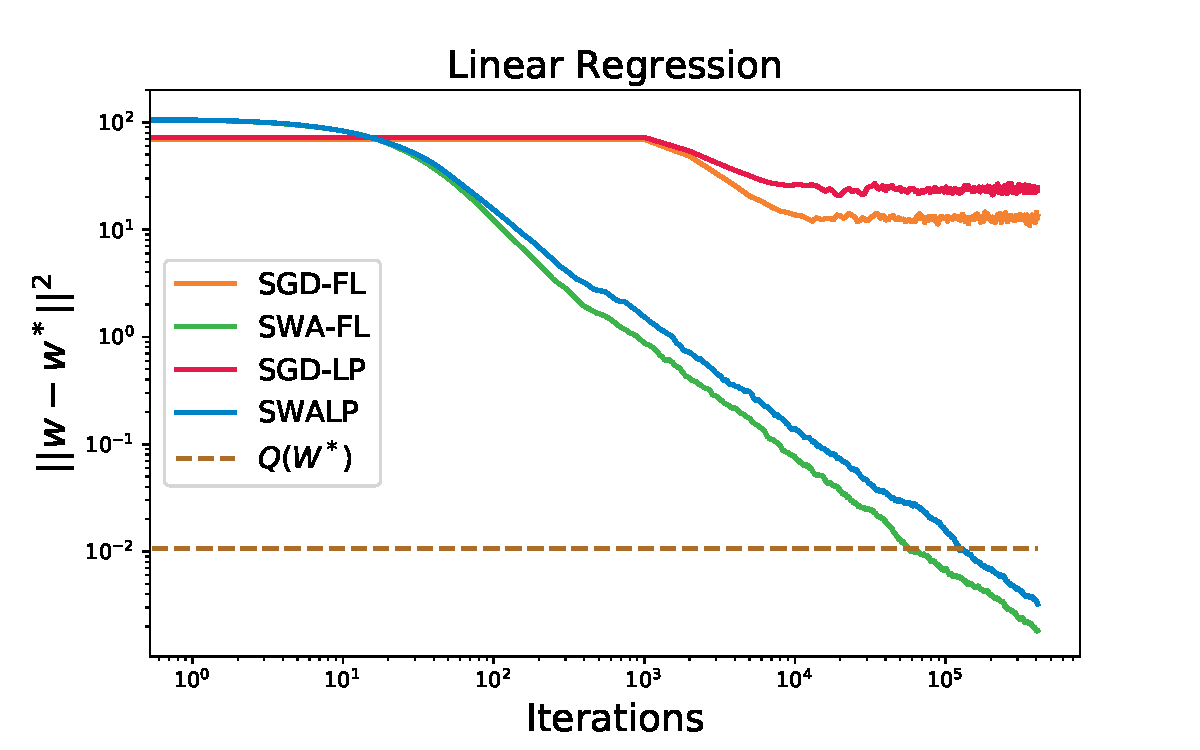
\includegraphics[width=0.4\textwidth]{figures/regression-log-log.pdf}\label{fig:log-log}
    }
    \subfigure[MNIST test error (\%) for logistic regression experiments. We varied the precisions used to train SGD-LP and SWALP.]{
        \centering
        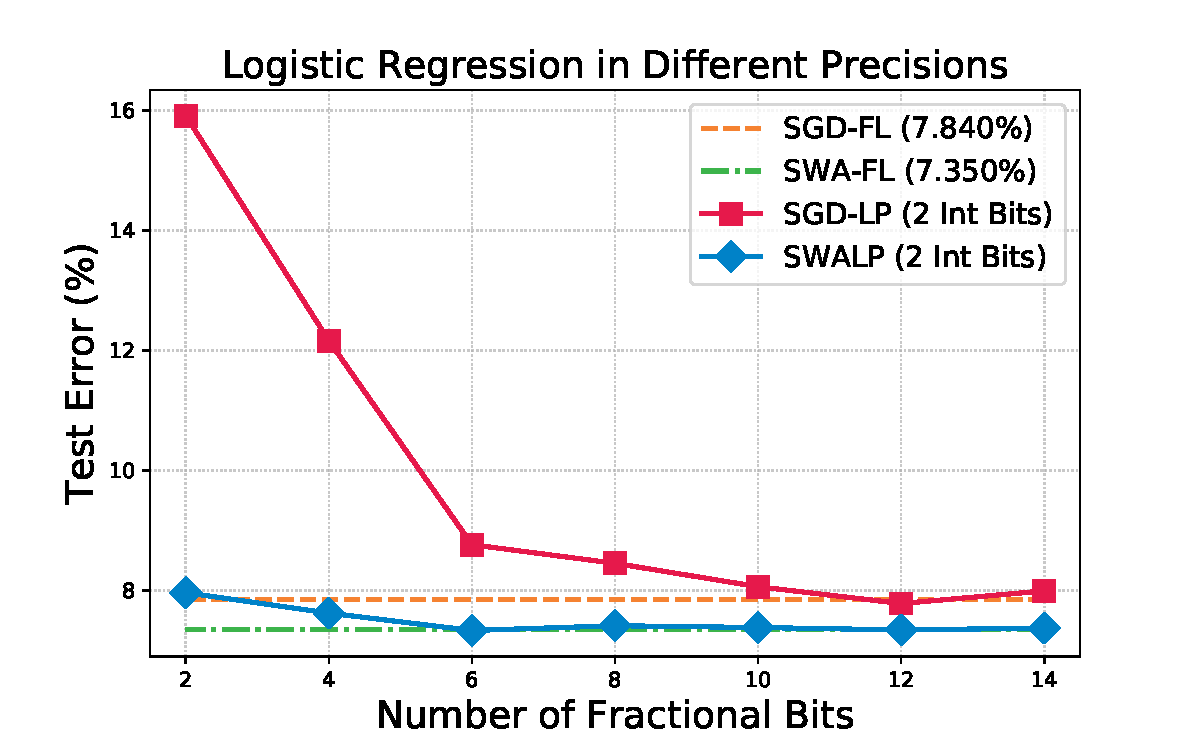
\includegraphics[width=0.45\textwidth]{figures/LogReg-Test-DiffBits.pdf}\label{fig:logreg-diff-prec-test}
    }
    \caption{More experimental results for linear and logistic regression.}
\end{figure*}


\textbf{Convergence.}
We plot the square distance between $w_t$ (or $\bar w_t$ for SWALP) and the optimal solution $w^*$ in log-log scale in Figure~\ref{fig:log-log}.
For reference, we also plot the squared distance between $Q(w^*)$ and $w^*$ to illustrate the size of quantization noise. It can be seen more clearly that the convergence rate is about $O(1/T)$.

\section{Implementation Details for Logistic Regression}\label{sec:logreg}

We use logistic regression with L2 regularization on MNIST dataset ~\cite{MNIST} .
In this experiment, we use the MNIST dataset~\cite{MNIST}. 
The objective function is defined as
$
    f(w) = - \frac{1}{n}\sum_{i=1}^n \log{(\operatorname{softmax}(w^Tx_i + b))} + \frac{\lambda}{2} \|w\|^2
$.
We choose $\lambda=10^{-4}$, a regularization parameter used in prior work~\cite{HALP,SVRG}, which makes the objective a strongly convex function with $M\ne 0$.
We use a learning rate of $\alpha = 0.01$ and cycle length $C=1$ for all four settings.
For this experiment we measure the norm of gradient at each iteration to illustrate the convergence of the algorithm; this is a more useful metric because MNIST is sparse and poorly conditioned, and it is a metric that has been used for logistic regression on MNIST in previous work~\cite{HALP}.
We warm up for 60000 iterations. 
For SWALP and SGD-LP, we use 4-bit word length and 2-bit fractional length.
For the experiment where we evaluate different precision, we use the same hyper-parameters, except the following: 1) the warm-up period is set to 600k iterations (i.e. 10 epochs); and 2) we report the final evaluation results after training for 3 million steps (i.e. 50 epochs). The test results is reported in Figure~\ref{fig:logreg-diff-prec-test}. As we could see the same conclusion still holds. Detail statistics is reported in Table~\ref{table:logreg-diffprec-stats}.

\begin{table}[H]
\centering
\caption{MNIST training and testing error (\%) for logistic regression experiment with different fractional bits for training.} 
\begin{tabular}{lccccc}

\toprule
 & & \multicolumn{2}{c}{SGD} & \multicolumn{2}{c}{SWA} \\
Format & Precision & Train Err   & Test Err  & Train Err   & Test Err  \\
\midrule
Float & 32 & 7.07 & 7.84 & 6.6 & 7.35 \\
\multirow{7}{*}{Fixed Point} & FL=14, WL=16 & 7.30 & 7.99 & 6.59 & 7.37 \\
 & FL=12, WL=14 & 7.18 & 7.78 & 6.59 & 7.34 \\
 & FL=10, WL=12 & 7.21 & 8.06 & 6.57 & 7.38 \\
 & FL=8, WL=10 & 7.82 & 8.45 & 6.61 & 7.41 \\
 & FL=6, WL=8 & 8.31 & 8.76 & 6.78 & 7.33 \\
 & FL=4, WL=6 & 11.64 & 12.16 & 7.21 & 7.62 \\
 & FL=2, WL=4 & 16.27 & 15.91 & 7.98 & 7.96 \\
\bottomrule
\end{tabular}
\label{table:logreg-diffprec-stats}
\end{table}

\section{Implementation Details for Section~\ref{sec:expr}}\label{sec:dlexp}
For VGG-16 and Pre-activation ResNet-164, we replicate the full precision baselines by using the publicly released implementation of SWA~\cite{SWA-repo}. Based on validation error, we discover that for low-precision training it is beneficial to decay the learning rate lower before SWA starts. Therefore, we follow the SGD learning rate schedule described in \citet{SWA} before SWALP starts. For ResNet-18 on ImageNet dataset, we follow the learning rate schedule described in \citet{resnet}.

We now disclose the specific hyperparameters.
\begin{itemize}
    \item For VGG-16 reported in \citet{SWA}, we use He's initialization \cite{he-init} and weight decay of \texttt{5e-4}. One budget is set to be $200$ epochs. For SGD-LP, we set the initial learning rate $\alpha_1=0.05$ for the first $0.5$ budget, and linearly decreased to $0.01 \alpha_1$ for $0.5-0.9$ budget, and keep the learning rate constant for $0.9-1.0$ budget. For SWALP, we use the same learning rate for the first $200$ epochs. We starts SWALP averaging at $200$th epoch and keep a constant learning rate $0.01$ with averaging frequency $c=1$ epoch. 
    \item For Preactivation ResNet-164, we use He's initialization \cite{he-init} and weight decay of \texttt{3e-4}. One budget is set to be $150$ epochs. For SGD, we use cycle length $C=1$ and set the initial learning rate $\alpha_1=0.1$ for the first $0.5$ budget, and linearly decreased to $0.01 \alpha_1$ for $0.5-0.9$ budget, and keep the learning rate constant for $0.9-1.0$ budget. For SWALP, we start averaging at $150$ epoch and keep a constant learning rate $0.01$ with averaging frequency $c=1$ epoch. Moreover, we found that possibly because low-precision training is less stable, it is better to average for less epochs. Therefore, we evaluate the full precision averaged model on a subset of the training set and report the performance of the model with lowest loss on this subset. 
    \item For ResNet-18 on ImageNet, we use weight decay \texttt{1e-4}. One budget is set to be 90 epochs. For both SGD and SGD-LP, we use initial learning rate $0.1$ and decay it by a factor of 10 every 30 epochs. For SWA and SWALP, we start averaging after 90 epochs with a constant learning rate of $0.001$ for SWA and $0.001$ for SWALP (obtained by a grid search). The averaging frequency is $c=1$ epochs. 
\end{itemize}
    
\clearpage
\section{Data for Figure~\ref{fig:diffc_qswa}}\label{sec:data-figure3}



\begin{table*}[h]
\label{table:figure3-data-diffc}

\caption{CIFAR100 classification error (\%) on test set. We use the same base model and average it with different frequency. Each column show how the SWA model perform on the test set during the training according to each averaging schedule. }
\centering
\begin{tabular}{@{}lllllllllllllll@{}}
\toprule
Epoch   & \multicolumn{2}{c}{1} & \multicolumn{2}{c}{5} & \multicolumn{2}{c}{10} & \multicolumn{2}{c}{50} & \multicolumn{2}{c}{80} & \multicolumn{2}{c}{90} & \multicolumn{2}{c}{100} \\
\#batch/avg & Error         & STD        & Error         & STD        & Error          & STD        & Error          & STD        & Error          & STD        & Error          & STD        & Error          & STD         \\ \midrule
1                 & 28.95       & 0.12       & 28.38       & 0.12       & 28.01        & 0.10       & 27.20        & 0.34       & 27.21        & 0.13       & 27.19        & 0.13       & 27.11        & 0.29        \\
2                 & 28.96       & 0.12       & 28.37       & 0.13       & 28.01        & 0.10       & 27.20        & 0.34       & 27.21        & 0.13       & 27.19        & 0.13       & 27.12        & 0.29        \\
20                & 28.96       & 0.24       & 28.32       & 0.12       & 28.02        & 0.04       & 27.20        & 0.33       & 27.21        & 0.11       & 27.20        & 0.15       & 27.14        & 0.28        \\
100               & 29.20       & 0.21       & 28.47       & 0.09       & 28.23        & 0.18       & 27.24        & 0.29       & 27.18        & 0.23       & 27.17        & 0.17       & 27.18        & 0.22        \\
200               & 29.63       & 0.31       & 28.74       & 0.15       & 28.25        & 0.14       & 27.27        & 0.29       & 27.23        & 0.21       & 27.17        & 0.14       & 27.20        & 0.20        \\
once/epoch                & 30.00       & 0.12       & 28.88       & 0.13       & 28.28        & 0.10       & 27.23        & 0.31       & 27.14        & 0.16       & 27.19        & 0.15       & 27.16        & 0.26        \\ \bottomrule
\end{tabular}
\end{table*}

\begin{table*}[h]
\label{table:figure3-data-qswa}
\caption{CIFAR100 classification error (\%) on test set. We use block floating point to quantize the average. Each column shows the result of using different number bits for the block floating point. }
\centering
\begin{tabular}{cccccccccc}
\toprule
\# of bits & Float            & 16               & 14               & 12               & 10               \\
Test Error & 26.65$\pm{0.29}$ & 26.65$\pm{0.29}$ & 26.66$\pm{0.29}$ & 26.65$\pm{0.29}$ & 26.60$\pm{0.33}$ \\
\midrule
\# of bits &  & 9                & 8                & 7                & 6 \\
Test Error &  & 26.67$\pm{0.28}$ & 26.85$\pm{0.38}$ & 27.48$\pm{0.38}$ & 29.48$\pm{0.25}$  \\
\bottomrule
\end{tabular}
\end{table*}


\end{appendices}
